Au cours de notre projet, nous devions implémenter un modèle de base de données conforme au modèle conceptuel imposé sur Moodle.


\definecolor{vert}{RGB}{0,128,0}

\newcommand{\ucode}[1]{\underline{\texttt{#1}}}

\section{Passage E/A \textrightarrow{} Modèle relationnel}

\subsection{Étapes générales}

\footnotesize
\begin{itemize}
  \item \textbf{Cas 1 :} Entité non‑faible  
  \item \textbf{Cas 2 :} Entité faible  
  \item \textbf{Cas 3 :} Associations $\langle1,1\rangle$  
  \item \textbf{Cas 4 :} Autres associations  
\end{itemize}

\subsection{Cas 1 : Entité non‑faible}
\begin{itemize}
  \item \texttt{Porte(}\ucode{nom\_porte}\texttt{, état)}  
  \item \texttt{Monde(}\ucode{nom\_monde}\texttt{)}  
  \item \texttt{JoueurHumain(}\ucode{nom\_joueur}\texttt{, ptsVie, ptsForce)}  
  \item \texttt{PiedDeBiche(}\ucode{nom\_pdb}\texttt{, estDéplaçable)}  
  \item \texttt{Pièce(}\ucode{nom\_piece}\texttt{)}  
\end{itemize}

\subsection{Cas 2 : Entité faible}
\begin{quote}
Aucune entité faible dans le modèle imposé.
\end{quote}

\subsection{Cas 3 : Associations $\langle1,1\rangle$}
Types d’associations
\begin{itemize}
  \item Contient (Monde–Porte)  
  \item Contient (Monde–Pièce)  
  \item Contient (Monde–JoueurHumain)  
  \item Contient (Pièce–JoueurHumain)  
\end{itemize}

Relations générées
\begin{itemize}
  \item \texttt{Porte(}\ucode{nom\_porte}\texttt{, état, }
        \textcolor{vert}{\ucode{nom\_monde}}\texttt{)}  
  \item \texttt{Monde(}\ucode{nom\_monde}\texttt{)}  
  \item \texttt{JoueurHumain(}\ucode{nom\_joueur}\texttt{, ptsVie, ptsForce, }
        \textcolor{vert}{\ucode{nom\_monde}}\texttt{, }
        \textcolor{vert}{\ucode{nom\_piece}}\texttt{)}  
  \item \texttt{PiedDeBiche(}\ucode{nom\_pdb}\texttt{, estDéplaçable)}  
  \item \texttt{Pièce(}\ucode{nom\_piece}\texttt{, }
        \textcolor{vert}{\ucode{nom\_monde}}\texttt{)}  
\end{itemize}

\subsection{Cas 4 : Autres associations}
\begin{itemize}
  \item \texttt{Possède\_Piece\_Porte(}\ucode{nom\_porte}\texttt{, }\ucode{nom\_piece}\texttt{, }\ucode{nom\_monde}\texttt{)}  
  \item \texttt{Contient\_Piece\_Pdb(}\ucode{nom\_piece}\texttt{, }\ucode{nom\_pdb}\texttt{, }\ucode{nom\_monde}\texttt{)}  
  \item \texttt{Possède\_Pdb\_JoueurHumain(}\ucode{nom\_pdb}\texttt{, }\ucode{nom\_joueur}\texttt{, }\ucode{nom\_monde}\texttt{, }\ucode{nom\_piece}\texttt{)}  
\end{itemize}

\normalsize



\section{Choix réalisés pour le modèle physique}

Pour faciliter l’implémentation du modèle physique tout en respectant les contraintes du projet, nous avons effectué plusieurs adaptations.

\paragraph{Ajout d’une clé étrangère dans la table \texttt{PiedDeBiche}:}  
Nous avons ajouté une clé étrangère \texttt{nom\_monde} à la table \texttt{PiedDeBiche}, ce qui donne la structure suivante :

\footnotesize
\begin{center}
\texttt{PiedDeBiche(}\ucode{nom\_pdb}\texttt{, estDéplaçable, \textcolor{vert}{\ucode{nom\_monde}})}
\end{center}
\normalsize

Cette clé permet, lors de la lecture de la base de données, d’identifier le monde auquel appartient un pied de biche et ainsi de retrouver précisément l’objet concerné.

\paragraph{Modification de l’association \texttt{Possède\_Piece\_Porte}:}  
Nous avons modifié la table représentant l’association \texttt{Possède\_Piece\_Porte} pour y inclure directement les deux pièces reliées par une porte. La nouvelle structure est la suivante :

\footnotesize
\begin{center}
\texttt{Possède\_Piece\_Porte(}\ucode{nom\_pieceA}\texttt{, }\ucode{nom\_pieceB}\texttt{, }\ucode{nom\_porte}\texttt{)}
\end{center}
\normalsize

Cette simplification permet une lecture plus directe de la base de données, en rendant explicite la relation entre les deux pièces et la porte qui les relis.

\section{Implémentation d'EnregistreurBD}

Pour l’implémentation de l’enregistreur, nous avons utilisé un \texttt{PreparedStatement} distinct pour chaque table SQL. Cela nous permet d’utiliser des requêtes SQL précompilées, ce qui améliore la performance de l’insertion des données.

Nous avons ensuite créé deux fonctions pour chaque type d’entité :

\footnotesize
\begin{itemize}
  \item \texttt{creerEntite} : ajoute une instance de l’entité à la base de données.
  \item \texttt{creerLesEntites} : appelle \texttt{creerEntite} pour ajouter toutes les entités d’un certain type.
\end{itemize}
\normalsize

\paragraph{Ordre d’insertion des entités}

Pour garantir la cohérence de la base de données, nous avons réfléchi à l’ordre dans lequel les entités devaient être insérées.

Logiquement, nous commençons par insérer \textbf{le monde}, car il contient la clé primaire utilisée comme clé étrangère dans les autres tables.

Ensuite, nous insérons les \textbf{pièces}, avant les \textbf{portes}. Pourquoi ce choix ? Car les portes sont contenues dans les pièces (chaque porte appartient à une pièce), il est donc nécessaire que les pièces soient déjà présentes dans la base.

Enfin, nous ajoutons les autres entités comme les joueurs humains et les objets (par exemple les pieds-de-biche).

\paragraph{Extraction des entités : portes, pièces, joueurs humains, pieds-de-biche}

Nous avions deux options pour extraire ces entités :
\begin{itemize}
  \item Ajouter des getters spécifiques dans la classe \texttt{Monde}.
  \item Utiliser les \textit{Streams} Java avec les méthodes \texttt{filter} et \texttt{map}.
\end{itemize}

Ne sachant pas si nous étions autorisés à modifier \texttt{Monde.java}, nous avons choisi d’utiliser le getter existant \texttt{monde.getEntites()} et de filtrer les entités via les \textit{Streams} :

\footnotesize
\begin{lstlisting}
List<Piece> pieces = entites.stream().filter(e -> e instanceof Piece)
                            .map(e -> (Piece) e)
                            .collect(Collectors.toList());

List<JoueurHumain> jhs = entites.stream().filter(e -> e instanceof JoueurHumain)
                                .map(e -> (JoueurHumain) e)
                                .collect(Collectors.toList());
\end{lstlisting}
\normalsize

Cependant, cette méthode implique de parcourir l’ensemble des entités à chaque fois, ce qui peut être inefficace. Une amélioration possible serait de \textit{parcourir la liste une seule fois}, et de répartir les entités dans plusieurs listes selon leur type. Cela permettrait de réduire la complexité de l’opération et d’optimiser les performances.


\section{Implémentation du LecteurBD}

L'implémentation nous a emmené à apporté les corrections nécessaires à la base de données que nous avons cités dans la section 2.2 . Ci-dessous, un exemple d'une table de la base de données: 
\begin{center}
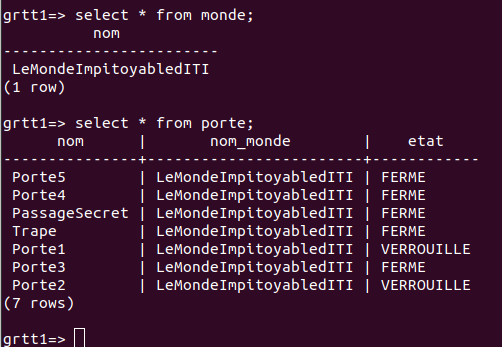
\includegraphics[height=3.5cm]{Persistance_BD/ressourcesBD/exemple_table.png}
\end{center}

\section{Amélioration possible}

Dans la partie base de données, nous aurions pu ajouter un attribut \texttt{ID} pour remplacer le rôle de clé étrangère actuellement joué par \texttt{nom\_monde}. En effet, le nom du monde étant une chaîne de caractères, il est dupliqué de nombreuses fois dans les différentes tables. Or, une chaîne de caractères occupe bien plus d’espace mémoire qu’un simple identifiant numérique. L’utilisation d’un \texttt{ID} permettrait donc d’optimiser l’espace mémoire et d’améliorer les performances des requêtes.


